\SourceLeaf{366}%
% A544-P0366-D01
Man kann nun beweisen
\begin{enumerate}\renewcommand{\labelenumi}{\arabic{enumi})}
\item Dass alle $\theta$, die aus (1) und aus (2) hervorgegangen sind, unter einander verschieden sind. Ihr Complexus heisse $\Theta$.
\item Dass alle $\theta=T+Ui$ die Eigenschaft haben, dass
\[
\begin{gathered}
-bT+aU\\
-BT+AU
\end{gathered}
\]
positive Zahlen kleiner als $\frac12\beta$ sind
\item Dass wenn $T,U$ zwei der eben genannten Bedingungen unterworfene ganze Zahlen sind, $T+Ui$ sich gewiss in $\Theta$ findet.\par
(wie denn? es wird auf obige Gleichung $^*$ gegründet.)
\item Auf ähnliche Weise verhält es sich mit $\theta'$, deren Complexus $\Theta'$ aus denjenigen Zahlen $T'+U'i$ bestehen wird, für welche
\[
\begin{gathered}
-bT'+aU'\\
-(-BT'+AU')
\end{gathered}
\]
positive Zahlen kleiner als $\frac12\beta$.
\end{enumerate}

% A544-P0366-D02
In unserm Falle ist
\[
\setlength{\arraycolsep}{4pt}
\begin{array}{r|r||r|r||r|r||r|r}
\theta&\varepsilon&\theta'&\varepsilon&\theta''&\varepsilon&\theta'''&\varepsilon\\
+1&+1&0+i&-1&+2-i&+1&+1&-1\\
+1+i&-1&0+2i&+1&+3-i&-1&+2&+1\\
+1+2i&+1&0+3i&-1&\multicolumn{4}{c}{}\\
\multicolumn{2}{c||}{}&-1+i&+1&\multicolumn{4}{c}{}\\
\multicolumn{2}{c||}{}&-1+2i&-1&\multicolumn{4}{c}{}\\
\multicolumn{2}{c||}{}&-1+3i&+1&\multicolumn{4}{c}{}
\end{array}
\]

% A544-P0366-D03
Hier ist
\[
\begin{aligned}
\theta&=-{}_*M+{}_*m\\
\theta'&=-{}_*M-{}_*m\\
\theta''&=+{}_*Mi+{}_*m\\
\theta'''&=+{}_*Mi-{}_*m
\end{aligned}
\]

\SourceLeaf{367}%
% A544-P0367-D01
\Article{10}
$3^0$. $y$ und $X$ Ganze. Es seien $x',Y'$ die nächsten Ganzen bei $x$ und $Y$, und
\[
x'+yi=p',\quad X+Y'i=P';\quad p-p'=\frac{p^0}{\alpha},\quad P-P'=\frac{P^0}{\alpha}
\]
und man setze
\[
\begin{aligned}
i(t+ui)&=Mp'-mP'=-\frac{Mp^0}{\alpha}+\frac{mP^0}{\alpha}\\
&=-\frac{Mx^0}{\alpha}+\frac{miY^0}{\alpha}\quad\text{d. i.}
\end{aligned}
\]
\[
\begin{alignedat}{3}
\alpha t&=-Bx^0+aY^0\quad&\text{so ist}\quad&x^0&=-bt+au\\
\alpha u&=+Ax^0+bY^0&&Y^0&=+At+Bu
\end{alignedat}
\]

% A544-P0367-D02
Man hat dann
\[
\varepsilon=-1,\text{ wenn }\alpha\text{ positiv, }x^0\text{ positiv, }Y^0\text{ positiv, }t+u\text{ gerade etc.}
\]
Wir setzen
\[
\begin{array}{rll}
&&\textit{besser}\\
t+ui=+\theta''&\text{wenn }x^0\text{ positiv, }Y^0\text{ positiv}&+\theta'\\
=+\theta'''&\text{wenn }x^0\text{ positiv, }Y^0\text{ negativ}&-\theta'''\\
-\theta''&\text{wenn }x^0\text{ negativ, }Y^0\text{ negativ}&-\theta'\\
-\theta'''&\text{wenn }x^0\text{ negativ, }Y^0\text{ positiv}&+\theta'''
\end{array}
\]
\[
\begin{array}{lr}
\text{Es wird also für jedes}&\theta''\pdot\pdot\pdot\;\varepsilon=-1\\
&\theta'''\pdot\pdot\pdot\;\varepsilon=+1
\end{array}
\]
insofern $\theta''$ oder $\theta'''$ durch $1+i$ theilbar und $\alpha$ positiv.

% A544-P0367-D03
\[
\setlength{\arraycolsep}{4pt}
\begin{array}{r|r|r|r|r|r|r|r}
y&X&x^0&X^0&t+ui&\theta''&\theta'''&\varepsilon\\
0&+1&+4&-2&+2&&+2&+1\\
+1&+2&-3&-3&-3+i&+3-i&&-1
\end{array}
\]

% A544-P0367-D04
\Article{11}
$4^{\mathrm{te}}$ Classe $x$ und $Y$ Ganze. Nach ähnlichen Praemissen wie in 3 setze man
\[
\begin{aligned}
-(t+ui)&=Mp'-mP'=-\frac{Mp^0}{\alpha}+\frac{mP^0}{\alpha}\\
&=-\frac{Miy^0}{\alpha}+\frac{mX^0}{\alpha}
\end{aligned}
\]
\[
\begin{alignedat}{2}
\alpha t&=-By^0-aX^0\qquad&y^0&=-bt+au\\
\alpha u&=+Ay^0-bX^0&X^0&=-At-Bu
\end{alignedat}
\]
Man hat dann
\[
\varepsilon=+1\text{ wenn }\alpha\text{ positiv, }y^0\text{ positiv, }X^0\text{ positiv, }t+u\text{ gerade etc.}
\]

\SourceLeaf{368}%
% A544-P0368-D01
Wir setzen
\[
\begin{array}{rl}
t+ui=+\theta''&\text{wenn }y^0\text{ positiv }X^0\text{ negativ}\\
+\theta'''&\text{wenn }y^0\text{ positiv }X^0\text{ positiv}\\
-\theta''&\text{wenn }y^0\text{ negativ }X^0\text{ positiv}\\
-\theta'''&\text{wenn }y^0\text{ negativ }X^0\text{ negativ}
\end{array}
\]
für $\varepsilon$ gilt dann die Regel, dass (wie oben in 3), insofern $\alpha$ positiv
\[
\begin{aligned}
\varepsilon=-1\text{ für jedes durch }1+i&\left\{\begin{array}{ll}\text{theilbare}&\theta''\\\text{untheilbare}&\theta'''\end{array}\right.\\[3pt]
\varepsilon=+1\text{ für jedes durch }1-i&\left\{\begin{array}{ll}\text{theilbare}&\theta'''\\\text{untheilbare}&\theta''\end{array}\right.
\end{aligned}
\]

% A544-P0368-D02
\[
\setlength{\arraycolsep}{4pt}
\begin{array}{r|r|r|r|r|r|r|r}
x&Y&y^0&X^0&t+ui&\theta''&\theta'''&\varepsilon\\
+1&-1&-2&-1&-1&&+1&-1\\
+2&-3&+1&-4&+2-i&+2-i&&+1
\end{array}
\]

% A544-P0368-D03
Der Complexus aller $\theta''$ aus 3 und 4, den wir durch $\Theta''$ bezeichnen, besteht also aus allen Zahlen $T+Ui$, wofür
\[
\left.\begin{array}{r}
-bT+aU\\
\text{und }+AT+BU
\end{array}\right\}\text{ positiv und kleiner als }\frac12\alpha
\]
der Complexus aller $\theta'''\pdot\pdot\pdot\;(\Theta''')$ aus denen, wo
\[
\left.\begin{array}{r}
-bT+aU\\
-AT-BU
\end{array}\right\}\text{ positiv und kleiner als }\frac12\alpha
\]

% A544-P0368-D04
\Article{12}
Nach obiger Verbesserung heisst also die Regel so:\par
Es enthalte
\[
\begin{aligned}
\Theta\quad&\text{alle Zahlen }T+Ui,\text{ wo }+bT-aU\text{ positiv}\\
&\quad -BT+AU\text{ positiv und }<\tfrac12\beta\\
\Theta'\quad&\text{alle Zahlen }T+Ui,\text{ wo }-bT+aU\text{ positiv}\\
&\quad +AT+BU\text{ positiv und }<\tfrac12\alpha\\
\Theta''\quad&\text{alle Zahlen }T+Ui,\text{ wo }-bT+aU\text{ positiv}\\
&\quad -BT+AU\text{ positiv und }<\tfrac12\beta\\
\Theta'''\quad&\text{alle Zahlen }T+Ui,\text{ wo }+bT-aU\text{ positiv}\\
&\quad +AT+BU\text{ positiv und }<\tfrac12\alpha
\end{aligned}
\]
insofern resp. $\beta$ oder $\alpha$ positiv.

\SourceLeaf{369}%
% A544-P0369-D01
\[
\begin{array}{c|c|l}
\text{Für alle durch}&\text{ist dann}&\text{wenn}\\
1+i\text{ theilbaren}&\varepsilon=&\\
\theta&+1&\beta\text{ positiv}\\
\theta'&-1&\alpha\text{ positiv}\\
\theta''&-1&\beta\text{ positiv}\\
\theta'''&+1&\alpha\text{ positiv}
\end{array}
\]

% A544-P0369-D02
\[
\setlength{\arraycolsep}{4pt}
\begin{array}{r|r||r|r||r|r||r|r}
\multicolumn{2}{c||}{\Theta}&\multicolumn{2}{c||}{\Theta'}&\multicolumn{2}{c||}{\Theta''}&\multicolumn{2}{c}{\Theta'''}\\
0-i&-1&+2-i&+1&+1&+1&-1&-1\\
0-2i&+1&+3-i&-1&+1+i&-1&-2&+1\\
0-3i&-1&\multicolumn{2}{c||}{}&+1+2i&+1&\multicolumn{2}{c}{}\\
+1-i&+1&\multicolumn{6}{c}{}\\
+1-2i&-1&\multicolumn{6}{c}{}\\
+1-3i&+1&\multicolumn{6}{c}{}
\end{array}
\]

% A544-P0369-D03
\begin{center}
\resizebox{.86\textwidth}{!}{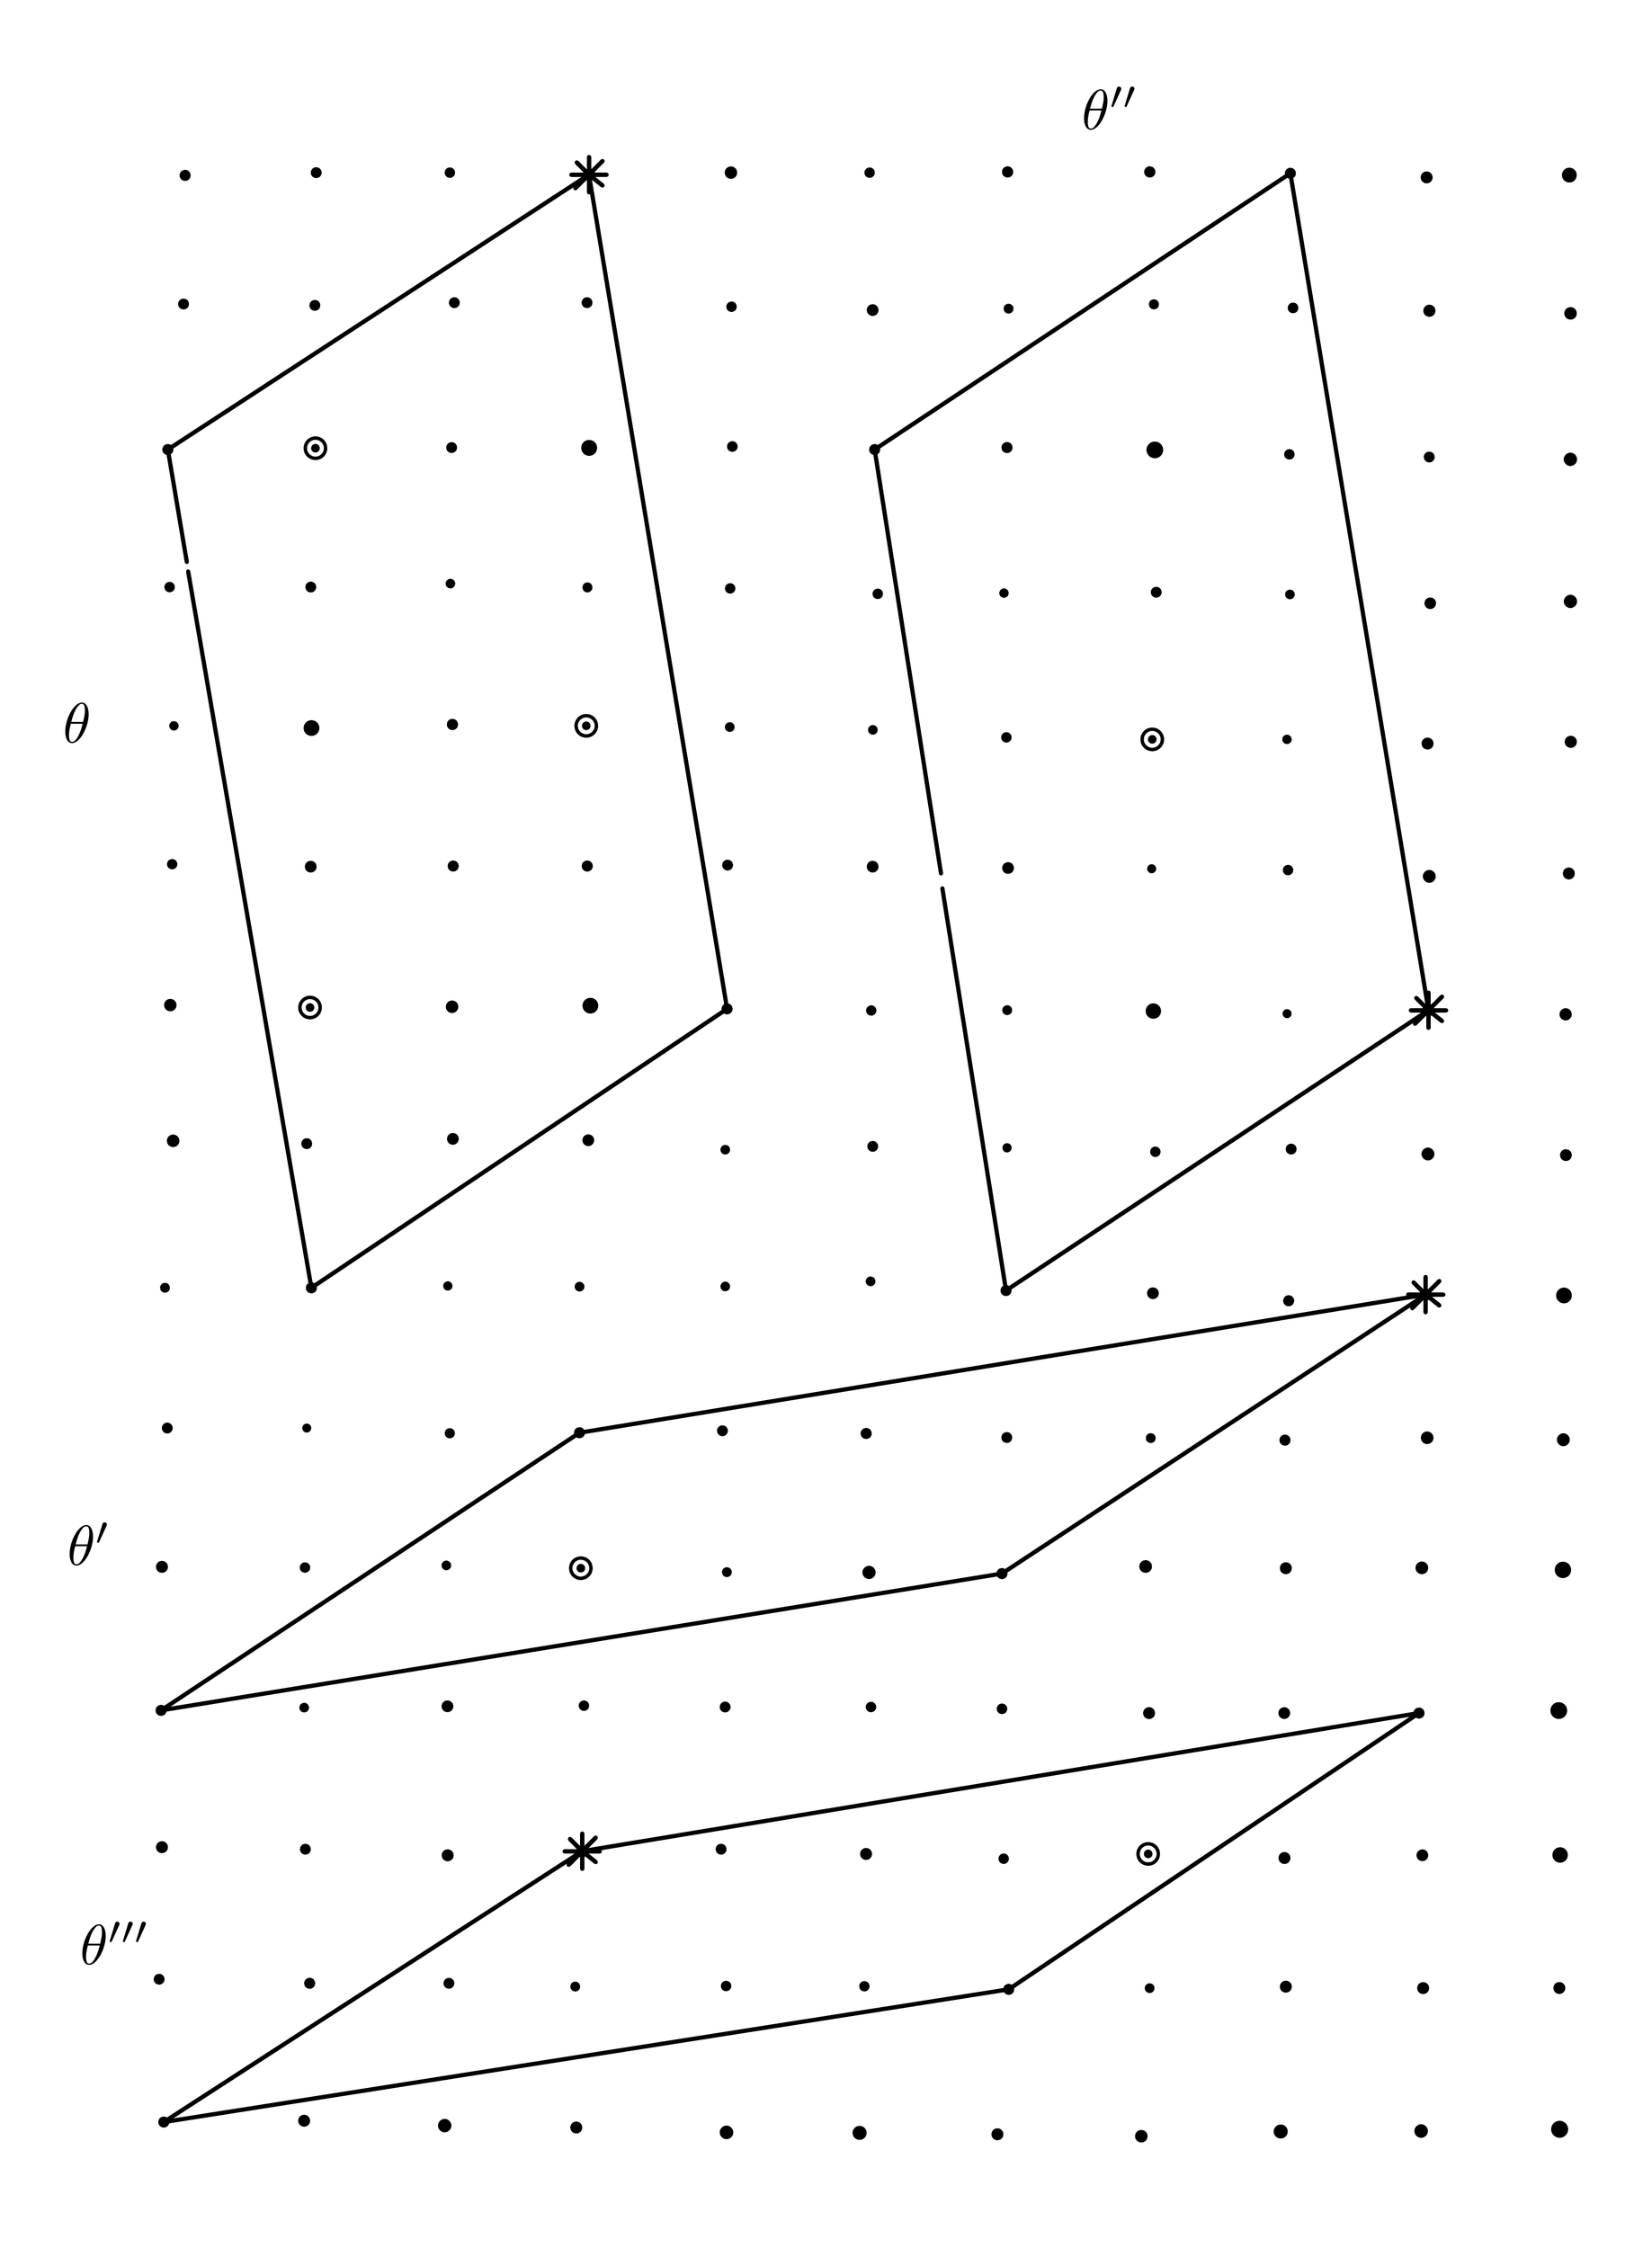
\begin{tikzpicture}[x=1bp,y=-1bp,line cap=round,line join=round]
\path[use as bounding box] (0,0) rectangle (1200,1640);
\begin{pgfinterruptboundingbox}
\draw[line width=3.1bp] (114,322) -- (425,119) -- (527,735) -- (220,941) -- (129,412);
\draw[line width=3.1bp] (128,405) -- (114,322);
\draw[line width=3.1bp] (636,322) -- (943,118) -- (1045,736) -- (733,943) -- (686,646);
\draw[line width=3.1bp] (685,635) -- (636,322);
\draw[line width=3.1bp] (109,1253) -- (418,1048) -- (1043,946) -- (730,1152) -- cycle;
\draw[line width=3.1bp] (111,1557) -- (420,1357) -- (1038,1255) -- (735,1459) -- cycle;
\fill (126.74,119.53) circle[radius=4.11bp];
\fill (223.57,117.53) circle[radius=4.03bp];
\fill (322.28,117.53) circle[radius=3.87bp];
\fill (425,119) circle[radius=4.5bp];
\draw[line width=3.2bp] (425,119) -- (425,106);
\draw[line width=3.2bp] (425,119) -- (435,109);
\draw[line width=3.2bp] (425,119) -- (438,119);
\draw[line width=3.2bp] (425,119) -- (435,127);
\draw[line width=3.2bp] (425,119) -- (425,132);
\draw[line width=3.2bp] (425,119) -- (415,129);
\draw[line width=3.2bp] (425,119) -- (412,119);
\draw[line width=3.2bp] (425,119) -- (416,110);
\fill (529.85,117.52) circle[radius=4.62bp];
\fill (632.28,117.53) circle[radius=3.87bp];
\fill (734.18,117.0) circle[radius=4.18bp];
\fill (839.18,117.0) circle[radius=4.18bp];
\fill (943,118) circle[radius=4.1bp];
\fill (1043.65,121.02) circle[radius=4.44bp];
\fill (1149.04,119.35) circle[radius=5.47bp];
\fill (125.57,214.53) circle[radius=4.03bp];
\fill (222.57,215.53) circle[radius=4.03bp];
\fill (325.57,213.53) circle[radius=4.03bp];
\fill (423.57,213.53) circle[radius=4.03bp];
\fill (530.28,216.53) circle[radius=3.87bp];
\fill (634.5,219.0) circle[radius=4.37bp];
\fill (734.88,217.95) circle[radius=3.66bp];
\fill (842.23,214.77) circle[radius=3.74bp];
\fill (944.98,217.41) circle[radius=3.95bp];
\fill (1045.66,219.5) circle[radius=4.51bp];
\fill (1149.91,221.44) circle[radius=4.65bp];
\fill (114,322) circle[radius=4.1bp];
\fill (223,321) circle[radius=3.2bp];
\draw[line width=2.5bp] (223,321) circle[radius=7.5bp];
\fill (323.57,320.53) circle[radius=4.03bp];
\fill (425.14,320.75) circle[radius=5.86bp];
\fill (530.88,319.73) circle[radius=3.95bp];
\fill (636,322) circle[radius=4.1bp];
\fill (733.74,320.53) circle[radius=4.11bp];
\fill (842.9,322.25) circle[radius=6.15bp];
\fill (942.28,325.53) circle[radius=3.87bp];
\fill (1045.57,327.53) circle[radius=4.03bp];
\fill (1149.8,329.21) circle[radius=4.92bp];
\fill (115.28,423.53) circle[radius=3.87bp];
\fill (219.57,423.53) circle[radius=4.03bp];
\fill (322.68,420.98) circle[radius=3.57bp];
\fill (423.88,423.79) circle[radius=3.7bp];
\fill (529.28,424.53) circle[radius=3.87bp];
\fill (638.28,428.53) circle[radius=3.87bp];
\fill (731.5,428.0) circle[radius=3.48bp];
\fill (843.94,427.35) circle[radius=4.03bp];
\fill (942.68,428.98) circle[radius=3.57bp];
\fill (1046.31,435.5) circle[radius=4.3bp];
\fill (1149.84,434.13) circle[radius=4.89bp];
\fill (118.5,526.0) circle[radius=3.48bp];
\fill (220.06,527.64) circle[radius=5.81bp];
\fill (324.18,525.0) circle[radius=4.18bp];
\fill (423,526) circle[radius=3.2bp];
\draw[line width=2.5bp] (423,526) circle[radius=7.5bp];
\fill (528.98,526.88) circle[radius=3.61bp];
\fill (634.67,528.98) circle[radius=3.57bp];
\fill (733.28,534.53) circle[radius=3.87bp];
\fill (841,536) circle[radius=3.2bp];
\draw[line width=2.5bp] (841,536) circle[radius=7.5bp];
\fill (940.5,536.0) circle[radius=3.48bp];
\fill (1044.31,539.1) circle[radius=4.44bp];
\fill (1150.09,537.81) circle[radius=4.51bp];
\fill (117.2,628.17) circle[radius=3.83bp];
\fill (219.5,630.0) circle[radius=4.37bp];
\fill (324.74,629.53) circle[radius=4.11bp];
\fill (423.74,629.53) circle[radius=4.11bp];
\fill (527.39,628.84) circle[radius=4.03bp];
\fill (634.5,630.0) circle[radius=4.37bp];
\fill (734.5,631.0) circle[radius=4.37bp];
\fill (840.57,631.54) circle[radius=3.34bp];
\fill (941.28,632.53) circle[radius=3.87bp];
\fill (1045.61,637.17) circle[radius=4.75bp];
\fill (1148.65,635.02) circle[radius=4.44bp];
\fill (115.82,732.21) circle[radius=4.62bp];
\fill (219,734) circle[radius=3.2bp];
\draw[line width=2.5bp] (219,734) circle[radius=7.5bp];
\fill (323.91,733.44) circle[radius=4.65bp];
\fill (426.06,732.64) circle[radius=5.81bp];
\fill (527,735) circle[radius=4.1bp];
\fill (633.46,736.2) circle[radius=3.83bp];
\fill (733.88,735.95) circle[radius=3.66bp];
\fill (841.81,736.62) circle[radius=5.67bp];
\fill (940.57,738.54) circle[radius=3.34bp];
\fill (1045,736) circle[radius=4.5bp];
\draw[line width=3.2bp] (1045,736) -- (1045,723);
\draw[line width=3.2bp] (1045,736) -- (1055,726);
\draw[line width=3.2bp] (1045,736) -- (1058,736);
\draw[line width=3.2bp] (1045,736) -- (1055,744);
\draw[line width=3.2bp] (1045,736) -- (1045,749);
\draw[line width=3.2bp] (1045,736) -- (1035,746);
\draw[line width=3.2bp] (1045,736) -- (1032,736);
\draw[line width=3.2bp] (1045,736) -- (1036,727);
\fill (1146.29,739.03) circle[radius=4.55bp];
\fill (117.91,832.44) circle[radius=4.65bp];
\fill (216.57,834.53) circle[radius=4.03bp];
\fill (324.5,831.0) circle[radius=4.37bp];
\fill (424.5,832.0) circle[radius=4.37bp];
\fill (525.67,838.98) circle[radius=3.57bp];
\fill (634.57,836.53) circle[radius=4.03bp];
\fill (733.76,837.59) circle[radius=3.43bp];
\fill (843.28,840.53) circle[radius=3.87bp];
\fill (943.57,838.53) circle[radius=4.03bp];
\fill (1044.61,842.17) circle[radius=4.75bp];
\fill (1146.5,843.0) circle[radius=4.37bp];
\fill (111.88,940.95) circle[radius=3.66bp];
\fill (220,941) circle[radius=4.1bp];
\fill (320.76,939.59) circle[radius=3.43bp];
\fill (418.05,940.12) circle[radius=3.61bp];
\fill (525.67,939.98) circle[radius=3.57bp];
\fill (632.98,936.2) circle[radius=3.61bp];
\fill (733,943) circle[radius=4.1bp];
\fill (841.5,945.0) circle[radius=4.37bp];
\fill (941.74,950.53) circle[radius=4.11bp];
\fill (1043,946) circle[radius=4.5bp];
\draw[line width=3.2bp] (1043,946) -- (1043,933);
\draw[line width=3.2bp] (1043,946) -- (1053,936);
\draw[line width=3.2bp] (1043,946) -- (1056,946);
\draw[line width=3.2bp] (1043,946) -- (1053,954);
\draw[line width=3.2bp] (1043,946) -- (1043,959);
\draw[line width=3.2bp] (1043,946) -- (1033,956);
\draw[line width=3.2bp] (1043,946) -- (1030,946);
\draw[line width=3.2bp] (1043,946) -- (1034,937);
\fill (1145.06,946.64) circle[radius=5.81bp];
\fill (113.57,1044.53) circle[radius=4.03bp];
\fill (216.57,1044.54) circle[radius=3.34bp];
\fill (322.22,1048.38) circle[radius=3.78bp];
\fill (418,1048) circle[radius=4.1bp];
\fill (523.57,1046.53) circle[radius=4.03bp];
\fill (629.74,1048.53) circle[radius=4.11bp];
\fill (733.57,1051.53) circle[radius=4.03bp];
\fill (839.88,1051.95) circle[radius=3.66bp];
\fill (939.02,1053.45) circle[radius=4.11bp];
\fill (1044.03,1051.71) circle[radius=4.69bp];
\fill (1144.61,1053.17) circle[radius=4.75bp];
\fill (109.65,1147.02) circle[radius=4.44bp];
\fill (215.28,1147.53) circle[radius=3.87bp];
\fill (319.68,1145.97) circle[radius=3.57bp];
\fill (419,1148) circle[radius=3.2bp];
\draw[line width=2.5bp] (419,1148) circle[radius=7.5bp];
\fill (526.88,1150.95) circle[radius=3.66bp];
\fill (631.84,1151.13) circle[radius=4.89bp];
\fill (730,1152) circle[radius=4.1bp];
\fill (836.11,1146.76) circle[radius=4.72bp];
\fill (939.65,1148.02) circle[radius=4.44bp];
\fill (1040.11,1147.76) circle[radius=4.72bp];
\fill (1144.3,1149.26) circle[radius=6.05bp];
\fill (109,1253) circle[radius=4.1bp];
\fill (214.68,1250.97) circle[radius=3.57bp];
\fill (320.5,1250.0) circle[radius=4.37bp];
\fill (421.28,1249.53) circle[radius=3.87bp];
\fill (525.57,1250.53) circle[radius=4.03bp];
\fill (633.28,1250.53) circle[radius=3.87bp];
\fill (730.02,1251.85) circle[radius=3.91bp];
\fill (838.65,1255.02) circle[radius=4.44bp];
\fill (938.5,1255.0) circle[radius=4.37bp];
\fill (1038,1255) circle[radius=4.1bp];
\fill (1141.22,1253.14) circle[radius=6.18bp];
\fill (109.65,1354.02) circle[radius=4.44bp];
\fill (215.57,1355.53) circle[radius=4.03bp];
\fill (320.65,1360.02) circle[radius=4.44bp];
\fill (420,1357) circle[radius=4.5bp];
\draw[line width=3.2bp] (420,1357) -- (420,1344);
\draw[line width=3.2bp] (420,1357) -- (430,1347);
\draw[line width=3.2bp] (420,1357) -- (433,1357);
\draw[line width=3.2bp] (420,1357) -- (430,1365);
\draw[line width=3.2bp] (420,1357) -- (420,1370);
\draw[line width=3.2bp] (420,1357) -- (410,1367);
\draw[line width=3.2bp] (420,1357) -- (407,1357);
\draw[line width=3.2bp] (420,1357) -- (411,1348);
\fill (522.57,1355.53) circle[radius=4.03bp];
\fill (629.65,1359.02) circle[radius=4.44bp];
\fill (731.28,1362.53) circle[radius=3.87bp];
\fill (838,1359) circle[radius=3.2bp];
\draw[line width=2.5bp] (838,1359) circle[radius=7.5bp];
\fill (938.65,1362.02) circle[radius=4.44bp];
\fill (1040.5,1360.0) circle[radius=4.37bp];
\fill (1142.22,1359.78) circle[radius=5.7bp];
\fill (107.57,1451.53) circle[radius=4.03bp];
\fill (218.74,1454.53) circle[radius=4.11bp];
\fill (321.57,1454.53) circle[radius=4.03bp];
\fill (414.88,1456.95) circle[radius=3.66bp];
\fill (526.28,1456.53) circle[radius=3.87bp];
\fill (628.41,1456.72) circle[radius=3.83bp];
\fill (735,1459) circle[radius=4.1bp];
\fill (839.05,1458.12) circle[radius=3.61bp];
\fill (939.65,1457.02) circle[radius=4.44bp];
\fill (1041.06,1458.08) circle[radius=4.44bp];
\fill (1141.65,1458.02) circle[radius=4.44bp];
\fill (111,1557) circle[radius=4.1bp];
\fill (214.65,1556.02) circle[radius=4.44bp];
\fill (318.44,1559.62) circle[radius=4.95bp];
\fill (415.65,1561.02) circle[radius=4.44bp];
\fill (526.58,1564.62) circle[radius=5.01bp];
\fill (624.87,1564.98) circle[radius=5.17bp];
\fill (726.65,1566.02) circle[radius=4.44bp];
\fill (832.91,1567.44) circle[radius=4.65bp];
\fill (935.87,1563.98) circle[radius=5.17bp];
\fill (1039.58,1563.62) circle[radius=5.01bp];
\fill (1141.86,1562.33) circle[radius=6.26bp];
\node[inner sep=0pt,outer sep=0pt,anchor=center] at (47,524) {\scalebox{4.2}{\ensuremath{\theta}}};
\node[inner sep=0pt,outer sep=0pt,anchor=center] at (56,1130) {\scalebox{4.2}{\ensuremath{\theta'}}};
\node[inner sep=0pt,outer sep=0pt,anchor=center] at (810,70) {\scalebox{4.2}{\ensuremath{\theta''}}};
\node[inner sep=0pt,outer sep=0pt,anchor=center] at (75,1425) {\scalebox{4.2}{\ensuremath{\theta'''}}};
\end{pgfinterruptboundingbox}
\end{tikzpicture}
}
\end{center}

\SourceLeaf{370}%
% A544-P0370-D01
\Article{13}
Hieraus fliesst folgende Regel. Es sei das Resultat aus den Vorschriften
\[
\mathrm{II}\pdot\pdot\pdot\;G,\quad
\mathrm{III}\pdot\pdot\pdot\;g,\quad
\mathrm{IV}\pdot\pdot\pdot\;H,\quad
\mathrm{V}\pdot\pdot\pdot\;h
\]
So ist
\[
\begin{aligned}
4\Theta&=R=0\\
4\Theta'&=-g+G-h-H+R'\\
4\Theta''&=-2g+2G+R''\\
4\Theta'''&=-g+G+h+H+R'''
\end{aligned}
\]

% A544-P0370-D02
In unserm Beispiele ist
\[
\begin{gathered}
G=0,\quad g=-1,\quad H=-1,\quad h=+2,\\
R'=0,\quad R''=+2,\quad R'''=-2\\
4\Theta=0,\quad4\Theta'=+1-1+0=0,\\
4\Theta''=+2+2=+4,\quad4\Theta'''=+1+1-2=0
\end{gathered}
\]
und die Correctionen $R,R'$ etc. werden so bestimmt: Es ist

% A544-P0370-D03
\[
R=\left\{\begin{array}{l}
-(\beta)+\frac12(\alpha\beta)+\frac12(\alpha\beta abAB)\\
-\frac12(b)-\frac12(B)\\
+(\beta)-\frac12(\alpha\beta)-\frac12(\alpha\beta abAB)\\
+\frac12(b)+\frac12(B)
\end{array}\right.
\]

% A544-P0370-D04
\[
R'=\left\{\begin{array}{l}
+(\alpha)-\frac12(\alpha\beta)+\frac12(\alpha\beta abAB)\\
-\frac12(b)-\frac12(A)\\
0\\
-\frac12(a)+\frac12(B)
\end{array}\right.
\]

% A544-P0370-D05
\[
R''=\left\{\begin{array}{l}
+(\beta)+\frac12(\alpha\beta)+\frac12(\alpha\beta abAB)\\
-\frac12(b)+\frac12(B)\\
+(\beta)+\frac12(\alpha\beta)+\frac12(\alpha\beta abAB)\\
-\frac12(b)+\frac12(B)
\end{array}\right.
\]

% A544-P0370-D06
\[
R'''=\left\{\begin{array}{l}
-(\alpha)-\frac12(\alpha\beta)+\frac12(\alpha\beta abAB)\\
-\frac12(b)+\frac12(A)\\
0\\
+\frac12(a)+\frac12(B)
\end{array}\right.
\]
wo die in Parenthese stehenden Grössen blos die Zeichen hergeben.

